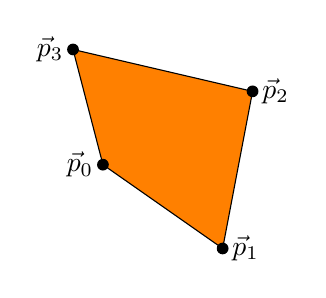
\begin{tikzpicture}[scale=1.9,yscale=0.7]
  \coordinate (zero) at (0, 0);
  \coordinate (one) at (0.8, -0.8);
  \coordinate (two) at (1, 0.7);
  \coordinate (three) at (-0.2, 1.1);
  \draw[fill=orange]
    (zero) node[left] {$\vec{p}_0$}
    -- (one) node[right] {$\vec{p}_1$}
    -- (two) node[right] {$\vec{p}_2$}
    -- (three) node[left] {$\vec{p}_3$}
    -- cycle;
  \foreach \n in {zero,one,two,three}
    \node at (\n)[circle,fill,inner sep=1.5pt]{};
\end{tikzpicture}
